\documentclass{beamer}
\usepackage{graphicx}
\usepackage{xcolor}
\usepackage{multirow}
%Information to be included in the title page:
\title{Toma Secuencial de Decisiones \newline y Aprendizaje por Refuerzo}
\author{Daniela Pucci de Farias}
\institute{Universidad Torcuato Di Tella}
\date{June 2025}

\begin{document}

\frame{\titlepage}

\begin{frame}{Contenidos del Curso}
\begin{itemize}
\item Modelado y resolución de problemas de toma de decisiones secuenciales
\begin{itemize}
\item<2-> Procesos markovianos de decisión
\item<2-> Aprendizaje por refuerzo
\end{itemize}
\item<3-> Cronograma:
\begin{itemize}
\item<4-> Clase 1: Introducción a toma de decisiones secuenciales y aprendizaje por refuerzo. Procesos markovianos. Aplicaciones al estudio de regímenes de mercado y análisis de participación de empresas en el mercado.

\item<5-> Clase 2: Procesos Markovianos con Recompensa y Procesos Markovianos de Decisión (MDP). MDPs con horizonte finito. Modelado y algoritmos. Aplicación a precificación dinámica.

\item<6-> Clase 3: MDPs con horizonte infinito. Modelado y algoritmos. Aplicación a optimización de portafolios.

\item<7-> Clase 4: Aprendizaje por refuerzo. Métodos computacionales exactos y por simulación.

\item<8-> Clase 5: Sistemas de larga escala. Métodos de aproximación. Aplicación a precificación de opciones americanas.
\end{itemize}
\end{itemize}   
\end{frame}

\begin{frame}{Horas de Consulta}
\begin{itemize}
\item Anteriormente a las clases teóricas, de 18 a 19h.
\item Ubicación:
\begin{itemize}
\item 2/6: Aula SV403 (4to piso, edificio Sáenz Valiente).
\item 9/6: Aula SV402 (4to piso, edificio Sáenz Valiente).
\item 23/6: Sala 4 (4to piso, edificio ALCORTA).
\item 30/6: Aula SV101 (1er piso, edificio Sáenz Valiente).
\item 7/7: Aula SV101 (1er piso, edificio Sáenz Valiente).
\end{itemize}
\end{itemize}
\end{frame}

\begin{frame}{Criterio de Evaluación}
La nota estará basada en el siguiente esquema de ponderación: 
\begin{itemize}
\item Participación en clase, asistencia y puntualidad: 10\%
\item<2-> Trabajo práctico grupal: 40\% 
\begin{itemize}
\item<3-> formación de los grupos: 9 de junio 
\item<3-> Propuesta de proyecto: 30 de junio
\item<3-> Presentación oral (15 minutos) y relatorio final: 31 de julio
\end{itemize}
\item<4-> Tareas individuales (2 tareas): 50\%
\begin{itemize}
\item<5-> Tarea 1: asignada el 2 de junio, fecha de entrega el 16 de junio
\item<5-> Tarea 2: asignada el 9 de junio, fecha de entrega el 23 de junio
\end{itemize}
\item<6-> Tareas y código python (Google Colab) deben ser entregados por el campus virtual
\end{itemize}
\end{frame}

\begin{frame}
\frametitle{Clase 1}
\begin{itemize}
\item<1-> Introducción a Toma de Decisiones Secuenciales y Aprendizaje por Refuerzo 
\item<2->Procesos Markovianos
\begin{itemize}
    \item Definición
    \item Propiedades
    \item Ejemplos
\end{itemize}
\end{itemize}
\end{frame}

\begin{frame}
\frametitle{Aprendizaje Automático (Machine Learning)}
    \centering
    \begin{tabular}{c@{\hskip 0.1cm}c}
        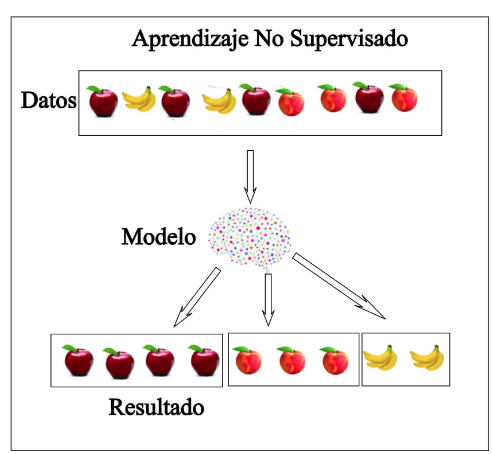
\includegraphics[width=0.45\textwidth]{../Images/MachineLearning/AprendizajeNoSupervisado.png} &
        \pause
        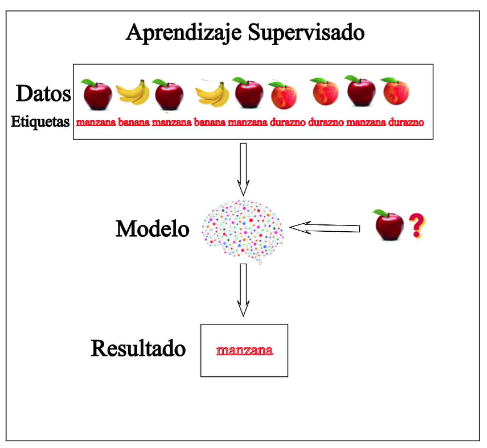
\includegraphics[width=0.45\textwidth]{../Images/MachineLearning/AprendizajeSupervisado.png} 
    \end{tabular}
\end{frame}

\begin{frame}
\frametitle{Aprendizaje Automático (Machine Learning)}
\begin{table}
    \centering
    \begin{tabular}{c@{\hskip 0.1cm}c}
        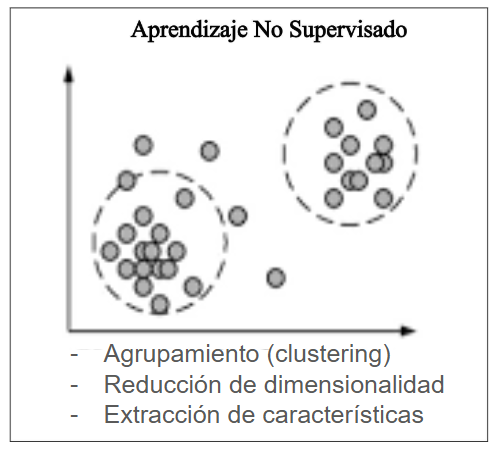
\includegraphics[width=0.45\textwidth]{../Images/MachineLearning/Clustering.png} &
        \pause
        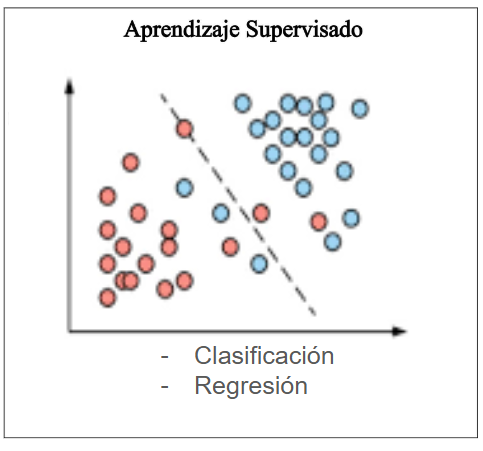
\includegraphics[width=0.45\textwidth]{../Images/MachineLearning/Clasificacion.png} 
    \end{tabular}
\end{table}
\end{frame}

\begin{frame}
\frametitle{Aprendizaje Por Refuerzo (Reinforcement Learning)}
 \centering
 \mode<beamer>{
    \only<1>{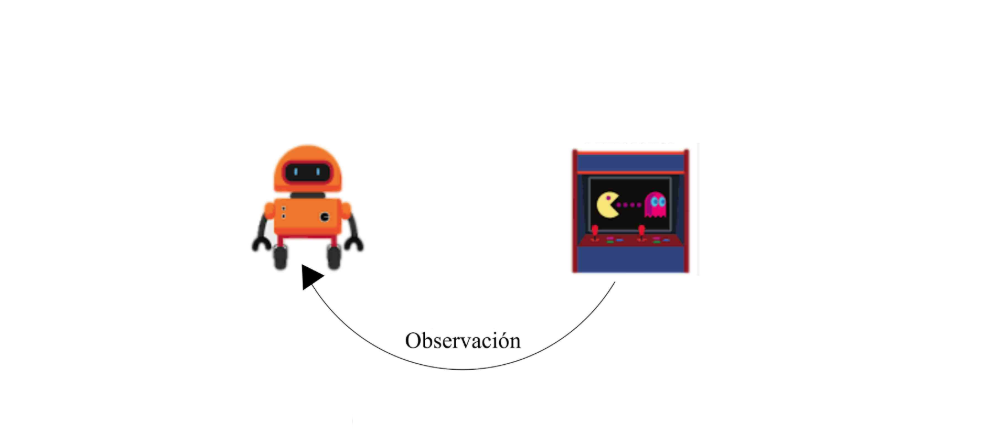
\includegraphics[width=1\textwidth]{../Images/RL/RL1.png}}
    \only<2>{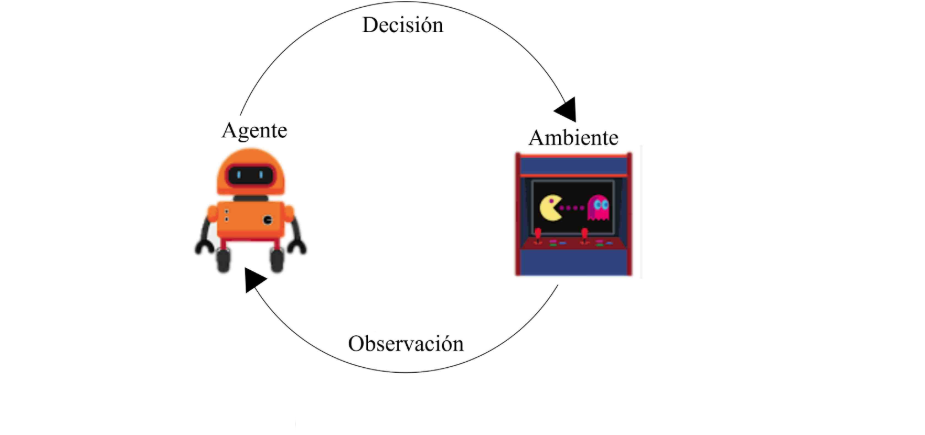
\includegraphics[width=1\textwidth]{../Images/RL/RL2.png}}}
    \only<3>{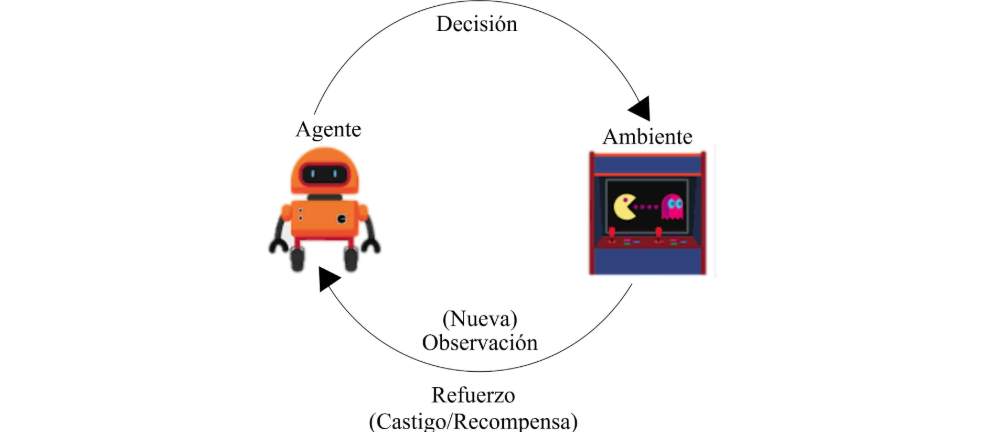
\includegraphics[width=1\textwidth]{../Images/RL/RL3.png}}
\end{frame}

\begin{frame}
\frametitle{Aprendizaje Por Refuerzo (Reinforcement Learning)}
\begin{itemize}
\item<1-> Aprendizaje de estrategias óptimas para situaciones que se extienden en el tiempo
\item<2-> La función de “refuerzo” puede ser diseñada para expresar diferentes objectivos
\item<3->Modelo de toma de decisiones secuenciales:
\begin{itemize}
    \item Ambiente tiene un estado que cambia al largo del tiempo 
    \item Evolución del estado afectada por decisiones
    \item Función de “refuerzo” afectada por estado y decisiones
\end{itemize}
\end{itemize}
\end{frame}

\begin{frame}
\frametitle{Aprendizaje Por Refuerzo (Reinforcement Learning)}
\begin{itemize}
\item<1-> Dificultades extras vs otros tipos de aprendizaje: 
\begin{itemize}
\item<2->Las consecuencias de una acción actual pueden impactar en el futuro
\begin{itemize}
\item<3-> No hay una señal directa midiendo ese impacto, solo la recompensa inmediata
\end{itemize}
\item<4-> El ambiente puede ser desconocido
\begin{itemize}
    \item<5-> Necesidad de aprender un modelo del ambiente y la acción
\end{itemize}
\item<6->Potencialmente muchas acciones posibles
\begin{itemize}
\item<7->
Hay que encontrar una forma eficiente de explorar las acciones
\end{itemize}
\end{itemize}
\end{itemize}
\end{frame}

\begin{frame}
\frametitle{Aprendizaje Por Refuerzo - Juegos}
\begin{table}
    \centering
    \begin{tabular}{c@{\hskip 0.1cm}c}
        TD-Gammon (1992) & \visible<2>{AlphaGo (2015-2017) }\\
        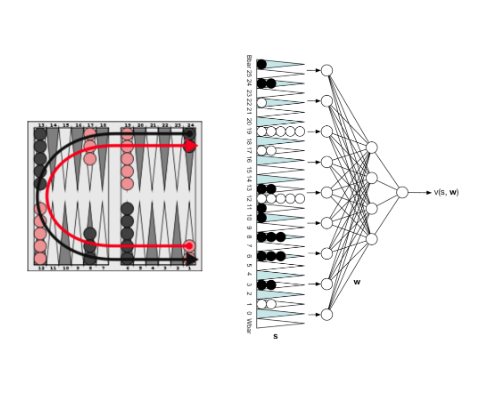
\includegraphics[width=0.45\textwidth]{../Images/RLExamples/TDGammon.png} & \visible<2>{
        
\includegraphics[width=0.45\textwidth] {../Images/RLExamples/AlphaGo.png}} 
    \end{tabular}
\end{table}
\end{frame}

\begin{frame}{Aprendizaje Por Refuerzo - Robótica}
    \centering
    \href{https://www.youtube.com/watch?v=DdojWYOK0Nc}
    {
        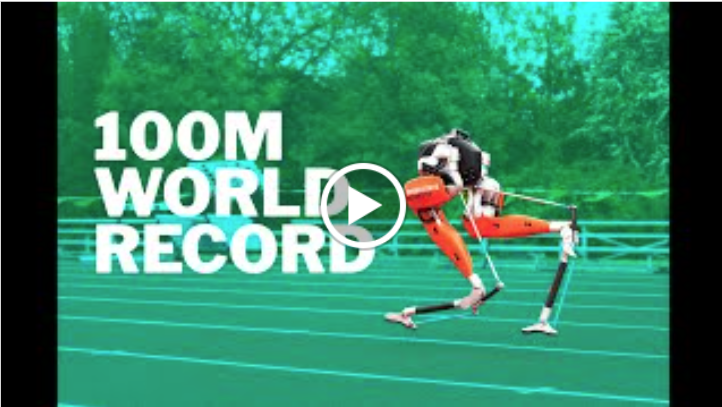
\includegraphics[width=0.9\textwidth]{../Images/RLExamples/Robotics.png}
    }
\end{frame}

\begin{frame}{Aprendizaje Por Refuerzo - Medicina}
    \centering
    
\includegraphics[width=0.9\textwidth]{../Images/Medicine/Medicine1.png}
\end{frame}

\begin{frame}{Aprendizaje Por Refuerzo - Medicina}
    \centering
    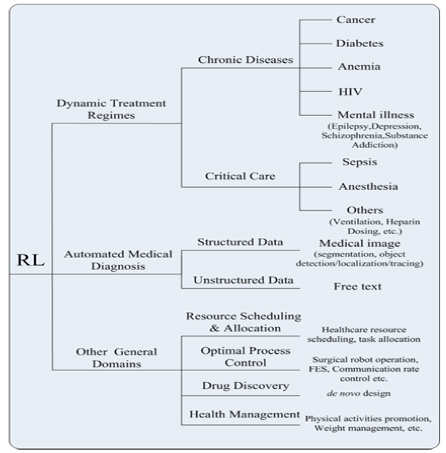
\includegraphics[width=0.7\textwidth]{../Images/Medicine/Medicine2.png}
\end{frame}

\begin{frame}{Aprendizaje Por Refuerzo - Procesamiento de Lenguaje Natural}
    \centering
    \begin{tabular}{c@{\hskip 0.4cm}c}
        
\includegraphics[width=0.5\textwidth]{../Images/NLP/NLP1.png} \\
        
\includegraphics[width=0.5\textwidth]{../Images/NLP/NLP2.png}
    \end{tabular}
\end{frame}   

\begin{frame}{Aprendizaje Por Refuerzo -
Vehículos Autónomos}
    \centering
    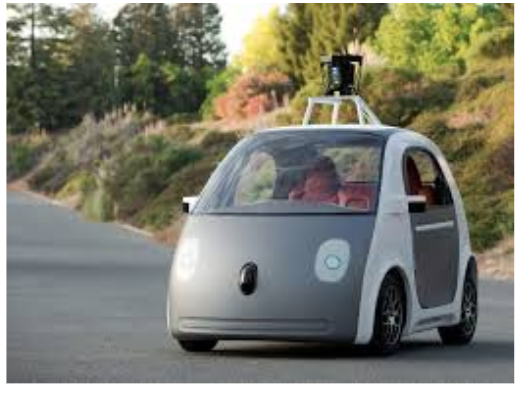
\includegraphics[width=0.7\textwidth]{../Images/RLExamples/AutonomousVehicle.png}
\end{frame}

\begin{frame}{Aprendizaje Por Refuerzo -
Sistemas de Energia}
    \centering
    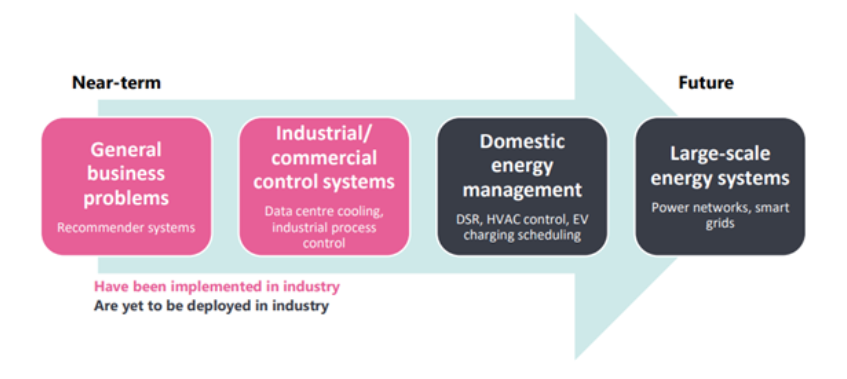
\includegraphics[width=0.7\textwidth]{../Images/RLExamples/EnergySystems.png}
\end{frame}

\begin{frame}{Aprendizaje Por Refuerzo}
\begin{itemize}
\item Marketing (campañas A/B, subastas)
\item Gestión de recursos 
\item Finanzas
\item Gestión de cadenas de suministro (supply chain management)
\item Precios dinámicos
\item …
\end{itemize}
\end{frame}

\begin{frame}{Toma Secuencial de Decisiones}
    \centering
    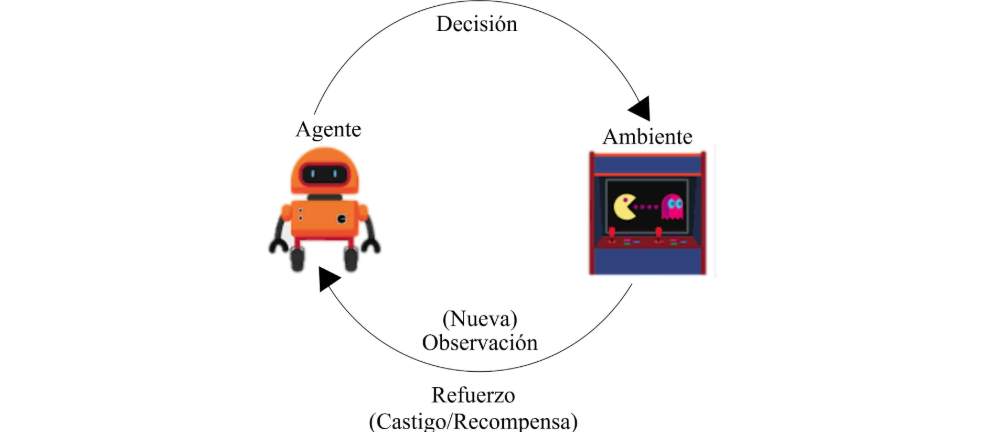
\includegraphics[width=0.8\textwidth]{../Images/RL/RL3.png}
    \begin{itemize}
        \item Cómo describir el problema matemáticamente?
        \item<2->Aprendizaje por refuerzo basado en Procesos de Decisión Markovianos
        (Markov Decision Processes - MDPs)
        \end{itemize}
\end{frame}

\begin{frame}{Procesos Markovianos}
\begin{itemize}
\item Ejemplo: cómo representar condiciones de mercado?
\item<2->En cada semana, uno de tres posibles estados
\item<3->Cómo evolucionan en el tiempo? 
\begin{itemize}
\item<4-> Descripción en términos de probabilidad
\item<6->En este curso, nos enfocaremos en procesos a tiempo discreto
\end{itemize}
\end{itemize}
\centering
\mode<beamer>{
\only<2>{
\includegraphics[width=0.95\textwidth]{../Images/Market/Market1.png}}
\only<3>{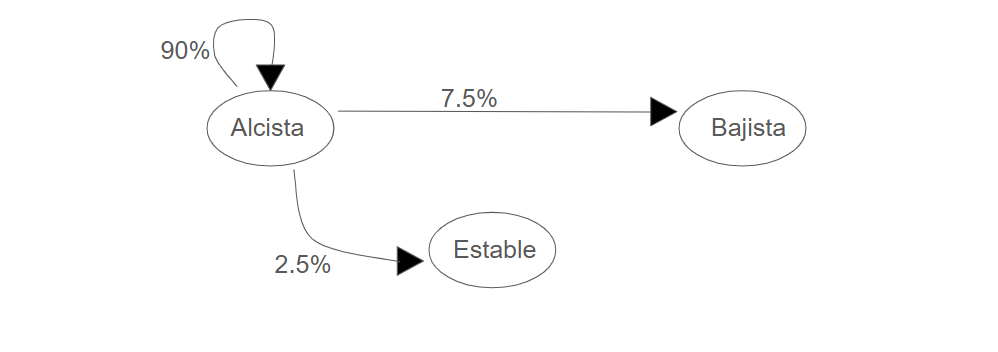
\includegraphics[width=0.95\textwidth]{../Images/Market/Market2.png}}
\only<4>{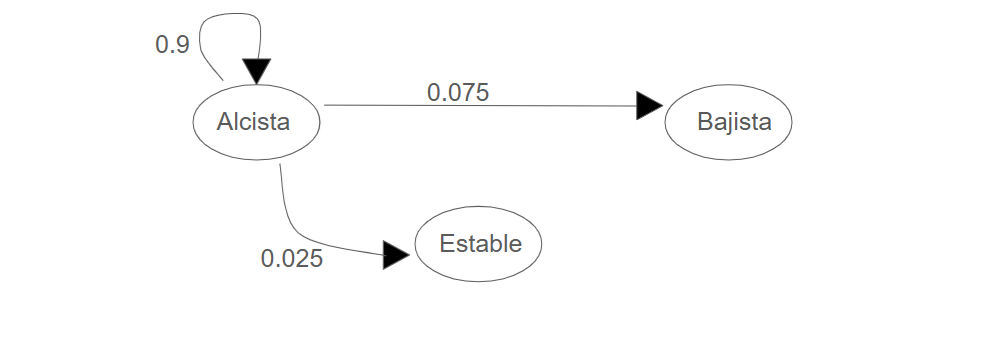
\includegraphics[width=0.95\textwidth]{../Images/Market/Market3.png}}
\visible<5->{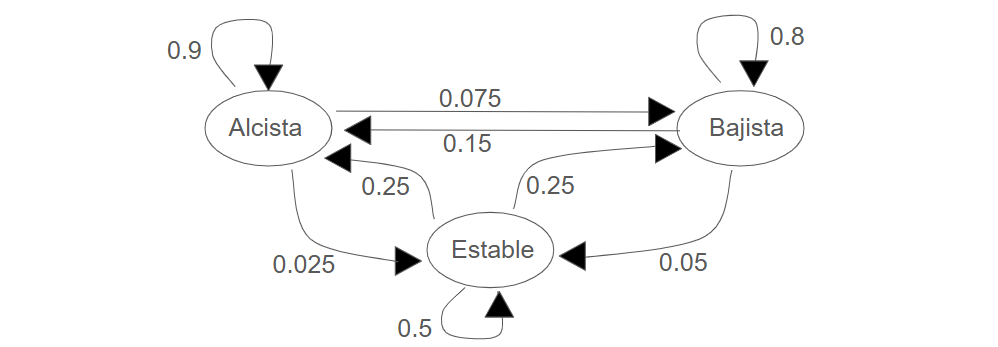
\includegraphics[width=0.95\textwidth]{../Images/Market/Market4.png}}}
\end{frame}

\begin{frame}{Procesos Markovianos}
Cómo definir matemáticamente el proceso de regímenes de mercado?
\begin{columns}[t]
\visible<2->{
\begin{column}[t]{0.6\textwidth}
\begin{itemize}
\item<2-> Espacio de estados $S$:
\begin{itemize}
    \item<2-> $S = \left\{\textbf{Alcista}, \textbf{Bajista}, \textbf{Estable}\right\}$
    \item<2-> Estados pueden ser discretos o continuos
\end{itemize}
\item<3-> Evolución en el tiempo
\mode<beamer>{
\only<3-7>{
\begin{tabular}{|c|c|c|c|}
\hline
    from/to & Alcista 2 & Bajista & Estable \\
    \hline
    Alcista & \visible<4-7>{0.9} &\visible<5-7>{0.075} & \visible<6-7>{0.025}  \\
    \hline
    Bajista & \visible<7>{0.15}&\visible<7>{0.8} & \visible<7>{0.05}  \\
    \hline
    Estable & \visible<7>{0.25}&\visible<7>{0.25} & \visible<7>{0.5} \\
    \hline    
\end{tabular}}}
\visible<8->{
\begin{itemize}
    \item Matriz de transición $P$: 
    $$P = \left[ 
    \begin{array}{ccc}
    0.9 & 0.075 & 0.025 \\
    0.15 & 0.8 & 0.05 \\
    0.25 & 0.25 & 0.5 \end{array}\right]$$
\end{itemize}}
\end{itemize}
\end{column}}
\begin{column}[t]{0.33\textwidth}
\mode<beamer>{
\only<1>{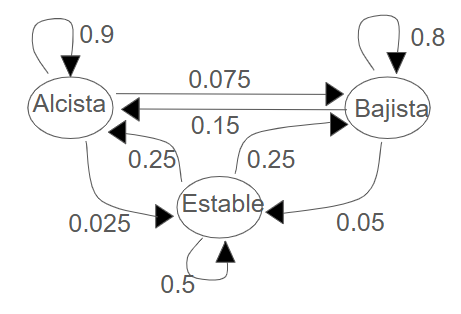
\includegraphics[width=1.1\textwidth]{../Images/MarkovProcess/MarkovProcess1.png}}
\only<2>{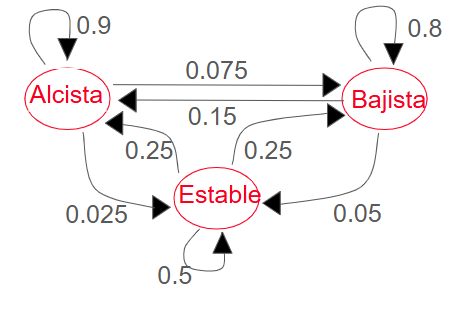
\includegraphics[width=1.1\textwidth]{../Images/MarkovProcess/MarkovProcess2.png}}
\only<3>{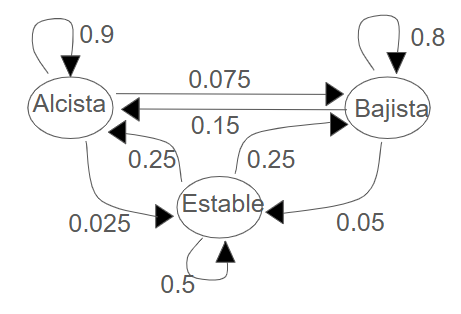
\includegraphics[width=1.1\textwidth]{../Images/MarkovProcess/MarkovProcess1.png}}
\only<4>{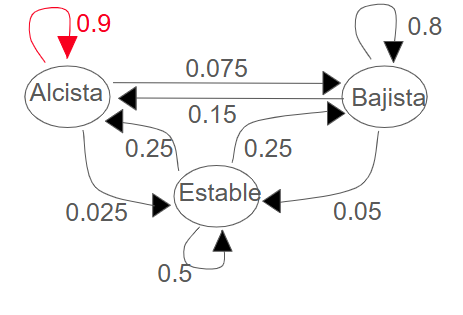
\includegraphics[width=1.1\textwidth]{../Images/MarkovProcess/MarkovProcess3.png}}
\only<5>{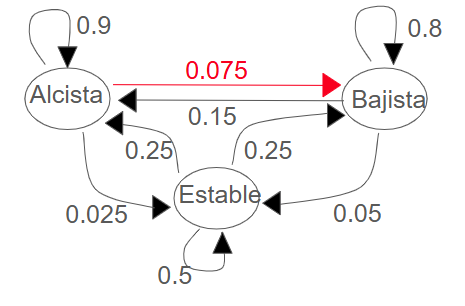
\includegraphics[width=1.1\textwidth]{../Images/MarkovProcess/MarkovProcess4.png}}
\only<6>{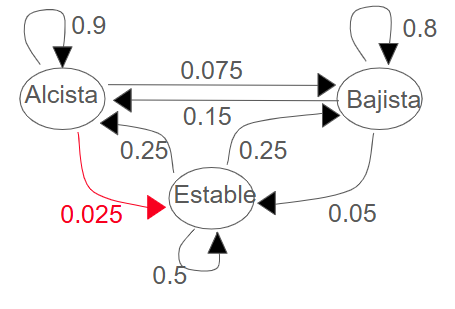
\includegraphics[width=1.1\textwidth]{../Images/MarkovProcess/MarkovProcess5.png}}}
\only<7->{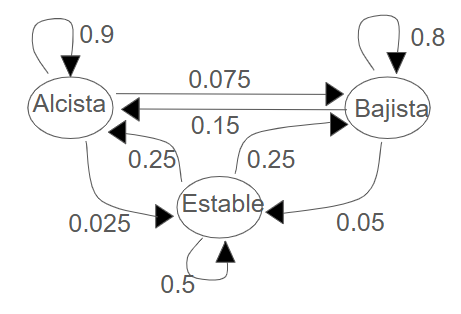
\includegraphics[width=1.1\textwidth]{../Images/MarkovProcess/MarkovProcess1.png}}
\end{column}
\end{columns}
\vspace{1em}
\visible<9->{
Tupla $(S,P)$ define el proceso markoviano
\begin{itemize}
    \item Si el número de estados es finito, también 
decimos cadena markoviana. 
\end{itemize}}
\end{frame}

\begin{frame}{Propiedad de Markov}
\begin{center}
\mbox{\hspace{-0.6cm}“El futuro del proceso markoviano depende solamente del estado presente.”}
\end{center}
\begin{itemize}
\item<2-> Proceso de Markov: tupla $(S,P)$
\item<3-> Estados  $s_0,~s_1,~s_2, \dots (s_t \in S ~{\rm for }~t = 0,1,2,\dots)$
\item<4-> ${\rm Prob}(s_{t+1}=s|s_0,s_1,...,s_t) = {\rm Prob}(s_{t+1}=s|s_t)$
\begin{itemize}
\item<5-> El estado st contiene toda la información relevante para el futuro del proceso
\item<5->Si conocemos $s_t$, podemos olvidar $s_{t-1}, ~s_{t-2},\dots,~s_0$.
\item<6->${\rm Prob}(s_{t+1}= s| s_t= s’) =   P(s,s’)$
\item<7-> Por ejemplo: 
$${\rm Prob}(s_{t+1}= \mathbf{Bajista} | s_t =\mathbf{Alcista}) = P(\mathbf{Alcista}, \mathbf{Bajista}) = 0.075$$
\end{itemize}
\end{itemize}
\end{frame}

\mode<beamer>{
\begin{frame}{Propiedad de Markov}
\begin{columns}[t]
\begin{column}[t]{0.6\textwidth}
\vspace{-2.5cm}
\only<1,2>{$$
\begin{array}{ccl} S & = & \left\{\textbf{Alcista}, \textbf{Bajista}, \textbf{Estable}\right\}\\
    P & = & \left[ 
    \begin{array}{ccc}
    0.9 & 0.075 & 0.025 \\
    0.15 & 0.8 & 0.05 \\
    0.25 & 0.25 & 0.5 \end{array}\right]
    \end{array}$$}
    \only<3>{$$
\begin{array}{ccl} S & = & \left\{\textbf{Alcista}, \textbf{Bajista}, \textbf{Estable}\right\}\\
    P & = & \left[ 
    \begin{array}{ccc}
    0.9 & \textcolor{red}{0.075} & 0.025 \\
    0.15 & 0.8 & 0.05 \\
    0.25 & 0.25 & 0.5 \end{array}\right]
    \end{array}$$}
\end{column}
\begin{column}{0.8\textwidth}
\only<1>{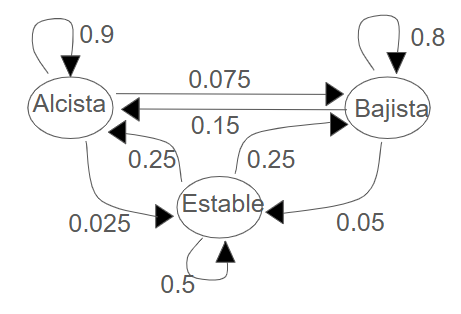
\includegraphics[width=0.4\textwidth]{../Images/MarkovProcess/MarkovProcess1.png}}
\only<2>{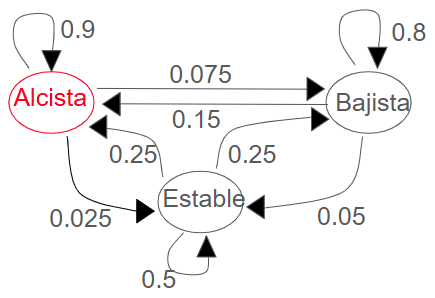
\includegraphics[width=0.4\textwidth]{../Images/MarkovProcess/MarkovProcess6.png}}
\only<3>{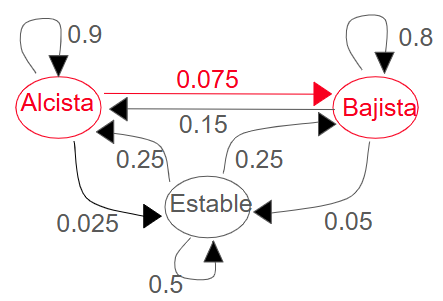
\includegraphics[width=0.4\textwidth]{../Images/MarkovProcess/MarkovProcess7.png}}
\end{column}
\end{columns}
Cuál es la probabilidad de tener un mercado \textbf {bajista en la próxima semana} 
\begin{enumerate} 
\item después de haber tenido un mercado \textbf {alcista en las últimas 5 semanas?}
\item después de haber tenido un mercado \textbf {alcista en la última semana, y bajista en las 4 anteriores?}
\end{enumerate}
\end{frame}}

\mode<handout>{
\begin{frame}{Propiedad de Markov}
\begin{columns}[t]
\begin{column}[t]{0.6\textwidth}
\vspace{-2.5cm}
    \only<3>{$$
\begin{array}{ccl} S & = & \left\{\textbf{Alcista}, \textbf{Bajista}, \textbf{Estable}\right\}\\
    P & = & \left[ 
    \begin{array}{ccc}
    0.9 & \textcolor{red}{0.075} & 0.025 \\
    0.15 & 0.8 & 0.05 \\
    0.25 & 0.25 & 0.5 \end{array}\right]
    \end{array}$$}
\end{column}
\begin{column}{0.8\textwidth}
\only<3>{
\includegraphics[width=0.4\textwidth]{MarkovProcess/MarkovProcess7.png}}
\end{column}
\end{columns}
Cuál es la probabilidad de tener un mercado \textbf {bajista en la próxima semana} 
\begin{enumerate} 
\item después de haber tenido un mercado \textbf {alcista en las últimas 5 semanas?}
\item después de haber tenido un mercado \textbf {alcista en la última semana, y bajista en las 4 anteriores?}
\end{enumerate}
\end{frame}}

\mode<beamer>{
\begin{frame}{Distribución Probabilística de Estados}
\begin{columns}[t]
\begin{column}[t]{0.6\textwidth}
\vspace{-2.5cm}
\only<1,3->{$$
\begin{array}{ccl} S & = & \left\{\textbf{Alcista}, \textbf{Bajista}, \textbf{Estable}\right\}\\
    P & = & \left[ 
    \begin{array}{ccc}
    0.9 & 0.075 & 0.025 \\
    0.15 & 0.8 & 0.05 \\
    0.25 & 0.25 & 0.5 \end{array}\right]
    \end{array}$$}
\only<2>{$$
\begin{array}{ccl} S & = & \left\{\textbf{Alcista}, \textbf{Bajista}, \textbf{Estable}\right\}\\
    P & = & \left[ 
    \begin{array}{ccc}
    0.9 & 0.075 & 0.025 \\
    0.15 & \textcolor{red}{0.8} & 0.05 \\
    0.25 & 0.25 & 0.5 \end{array}\right]
    \end{array}$$}
\end{column}
\begin{column}{0.8\textwidth}
\only<1,3->{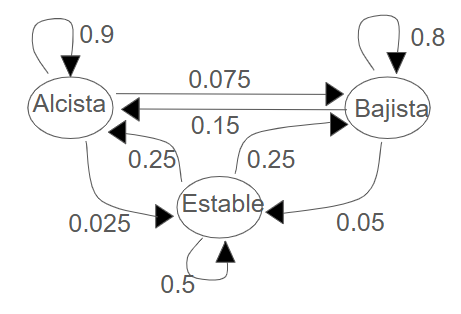
\includegraphics[width=0.4\textwidth]{../Images/MarkovProcess/MarkovProcess1.png}}
\only<2>{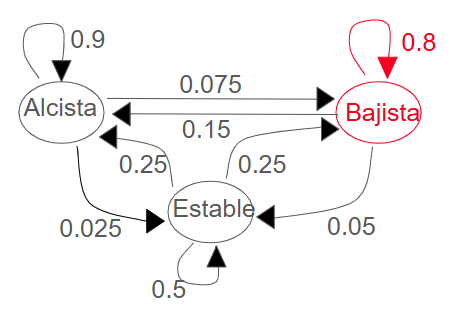
\includegraphics[width=0.4\textwidth]{../Images/MarkovProcess/MarkovProcess8.png}}
\end{column}
\end{columns}
\only<1>{Si esta semana el mercado es bajista, cuál es la probabilidad de que sea bajista en la próxima semana? En 2 semanas? En 10 semanas?}
\only<2>{Si esta semana el mercado es bajista, \textbf {cuál es la probabilidad de que sea bajista en la próxima semana?} En 2 semanas? En 10 semanas?}
\only<3-6>{Si esta semana el mercado es bajista, cuál es la probabilidad de que sea bajista en la próxima semana? \textbf{En 2 semanas?} En 10 semanas?}
\only<7,8>{Si esta semana el mercado es bajista, cuál es la probabilidad de que sea bajista en la próxima semana? En 2 semanas? \textbf{En 10 semanas?}}
\begin{itemize}
\only<2>{
\item La probabilidad de que sea bajista en la próxima semana es 0.8.}
\item<4-6> Podemos enumerar las posibilidades y sumarlas…
\only<5,6>{${\rm Prob}(\mathbf{Alcista}, \mathbf{Bajista}) + {\rm Prob}(\mathbf{Bajista}, \mathbf{Bajista}) + {\rm Prob}(\mathbf{Estable}, \mathbf{Bajista})$}
\only<6>{
	$ = 0.15*0.075 + 0.8*0.8 + 0.05*0.25$
    
	$= 0.66375$}
\item<8> Se puede responder a esas preguntas más fácilmente con álgebra linear!    
\end{itemize}
\end{frame}}

\mode<handout>{
\begin{frame}{Distribución Probabilística de Estados}
\begin{columns}[t]
\begin{column}[t]{0.6\textwidth}
\vspace{-2.5cm}
$$
\begin{array}{ccl} S & = & \left\{\textbf{Alcista}, \textbf{Bajista}, \textbf{Estable}\right\}\\
    P & = & \left[ 
    \begin{array}{ccc}
    0.9 & 0.075 & 0.025 \\
    0.15 & 0.8 & 0.05 \\
    0.25 & 0.25 & 0.5 \end{array}\right]
    \end{array}$$
\end{column}
\begin{column}{0.8\textwidth}
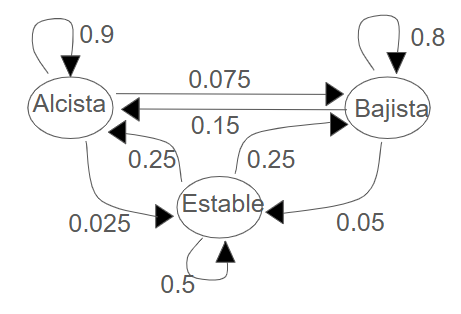
\includegraphics[width=0.4\textwidth]{../Images/MarkovProcess/MarkovProcess1.png}
\end{column}
\end{columns}
Si esta semana el mercado es bajista, cuál es la probabilidad de que sea bajista en la próxima semana? En 2 semanas? En 10 semanas?
\begin{itemize}
\item Se puede responder a esas preguntas más fácilmente con álgebra linear!    
\end{itemize}
\end{frame}}

\begin{frame}{Distribución Probabilística de Estados}

Vamos a representar una distribución probabilística de estados con la variable $\pi_t$: 

$$\pi_t(s) = {\rm Prob}(s_t = s).$$

\visible<2->{En nuestro ejemplo, si consideramos que esta semana corresponde a $t = 0$, tenemos ${\rm Prob}(s_0 = \mathbf{Altista}) = 0,~{\rm Prob}(s_0 = \mathbf{Bajista}) = 1),~{\rm Prob}(s_0 = \mathbf{Estable}) = 0.$}

\visible<3->{Entonces: 
$$
\pi_0 =\left[
\begin{array}{ccc}
0 & 1 & 0
\end{array}\right]$$}

\visible<4->{$\pi_0$ es la distribución inicial de estados en el proceso markoviano. } 
\visible<5>{
\begin{alertblock}{Resulta que $\pi_{t+1} = \pi_t P$  y  $\pi_t = \pi_0 P^t$.}
\end{alertblock}
}
\end{frame}

\begin{frame}{Distribución Probabilística de Estados}

Si esta semana el mercado es bajista, cuál es la probabilidad de que sea bajista en la próxima semana? En 2 semanas? En 10 semanas? 
\visible<2->{
\begin{alertblock}{Resulta que $\pi_t = \pi_0 P^t$.}
\end{alertblock}
}
\only<2>{
$$
\begin{array}{ccl}
\pi_1 & = & \pi_0 P \\
& = & \left[
\begin{array}{ccc}
0 & 1 & 0
\end{array}\right]\left[ 
    \begin{array}{ccc}
    0.9 & 0.075 & 0.025 \\
    0.15 & 0.8 & 0.05 \\
    0.25 & 0.25 & 0.5 \end{array}\right] \\
    & = & \left[\begin{array}{ccc}
0.15 & \textcolor{red}{0.8} & 0.05
\end{array}\right]
\end{array}$$
${\rm Prob}(s_1 = \textbf{Bajista}| s_0 = \textbf{Bajista}) = 0.8$
}
\only<3>{
$$
\begin{array}{ccl}
\pi_2 & = & \pi_0 P^2 \\
& = & \left[
\begin{array}{ccc}
0 & 1 & 0
\end{array}\right]\left[ 
    \begin{array}{ccc}
    0.9 & 0.075 & 0.025 \\
    0.15 & 0.8 & 0.05 \\
    0.25 & 0.25 & 0.5 \end{array}\right]^2 \\
    & = & \left[ \begin{array}{ccc}
0.2675 & \textcolor{red}{0.66375} & 0.06875
\end{array}\right]
\end{array}$$
${\rm Prob}(s_2 = \textbf{Bajista}| s_0 = \textbf{Bajista}) = 0.66375$
}
\only<4>{
$$
\begin{array}{ccl}
\pi_{10} & = & \pi_0 P^{10} \\
& = & \left[
\begin{array}{ccc}
0 & 1 & 0
\end{array}\right]\left[ 
    \begin{array}{ccc}
    0.9 & 0.075 & 0.025 \\
    0.15 & 0.8 & 0.05 \\
    0.25 & 0.25 & 0.5 \end{array}\right]^{10} \\
    & = & \left[ \begin{array}{ccc}
0.59159 & \textcolor{red}{0.34310} & 0.06532
\end{array}\right]
\end{array}$$
${\rm Prob}(s_10 = \textbf{Bajista}| s_0 = \textbf{Bajista}) = 0.34310$
}
\end{frame}

\begin{frame}{Distribución Probabilística de Estados}

Cuál es la frecuencia de semanas alcistas, bajistas y estables en ese mercado?

\visible<2->{Buscamos la \textbf{distribución estacionaria} de ese proceso.}
\begin{itemize}
    \item<3-> Tenemos $\pi_{t+1} = \pi_t x P$ y estacionariedad implica $\pi_{t+1} = \pi_t = \pi$.
    \item<4-> Queremos resolver \textcolor{red}{$\pi = \pi P$.}
    \item<5-> Si el número de estados es finito, siempre existe una solución, pero no es necesariamente única.
\end{itemize}
\visible<6->{
$$\begin{array}{ccl}
\pi_\infty & = & \pi_0 P^\infty \\
& = & \left[
\begin{array}{ccc}
0 & 1 & 0
\end{array}\right]\left[ 
    \begin{array}{ccc}
    0.9 & 0.075 & 0.025 \\
    0.15 & 0.8 & 0.05 \\
    0.25 & 0.25 & 0.5 \end{array}\right]^\infty \\
    & \approx & \left[ \begin{array}{ccc}
0.625 & \textcolor{red}{0.3125} & 0.0625
\end{array}\right]
\end{array}$$
}
\visible<7>{
\textbf{En ese mercado, 62.5\% de las semanas son alcistas, 31.25\% son bajistas, y 6.25\% son estables.}
}
\end{frame}
\begin{frame}{Ejemplo: Google PageRank}
Cuando hacemos una búsqueda en Google, las páginas que satisfacen a nuestras condiciones son presentadas en orden de importancia.

Cómo determinar importancia/ranking?
\mode<beamer>{
\includegraphics<2>[width=1.1\textwidth]{../Images/PageRank/PageRank1.png}}
\includegraphics<3>[width=1.1\textwidth]{../Images/PageRank/PageRank2.png}
\end{frame}

\begin{frame}{Ejemplo: Participación en El Mercado}

Cadenas markovianas son frecuentemente utilizadas para modelar el comportamiento de usuarios de proveedores adversarios y predecir la participación en el mercado de esos proveedores al largo del tiempo.
\begin{itemize}
\item<2>$p_{ij} $= probabilidad que usuario de proveedor $i$ cambie a proveedor $j$ 
\end{itemize}
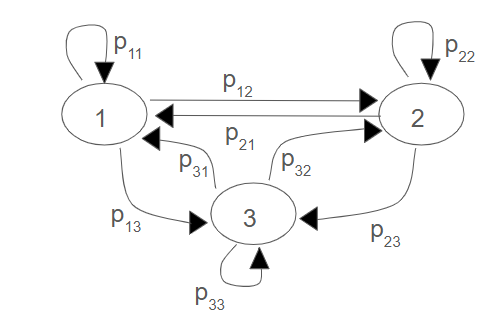
\includegraphics[width=0.8\textwidth]{../Images/RLExamples/MarketCompetition.png}
\end{frame}

\begin{frame}{Ejemplo: Participación en El Mercado}
\begin{center}
\textbf{Table 4: Respondents Brand Switching Behavior}
\only<1>{
\begin{tabular}{|c|c|c|c|c|c|c|c|}
\hline
\multirow{2}{*}{\textbf{Gains and Losses}} & \multicolumn{6}{|c|}{\textbf{Mobile Telecom Operators}} & \multirow{2}{*}{\textbf{Total}}  \\
&\textbf{M} & \textbf{V} & \textbf{T} & \textbf{E} & \textbf{A} & \textbf{G} & \\ \hline
\textbf{M} & 290 & 38 & 24 & 2 & 36 & 15 & \textbf{405} \\
\hline
\textbf{V} & 80 & 91 & 22 & 4 & 32 & 6 & \textbf{235} \\
\hline
\textbf{T} & 83 & 17 & 101 & 4 & 21 & 11 & \textbf{237} \\
\hline
\textbf{E} & 9 & 6 & 11 & 4 & 0 & 0 & \textbf{30} \\
\hline
\textbf{A} & 72 & 22 & 21 & 2 & 87 & 5 & \textbf{209} \\
\hline
\textbf{G} & 38 & 9 & 13 & 1 & 21 & 32 & \textbf{114} \\
\hline
\end{tabular}}
\mode<beamer>{
\only<2>{
\begin{tabular}{|c|c|c|c|c|c|c|c|}
\hline
\multirow{2}{*}{\textbf{Gains and Losses}} & \multicolumn{6}{|c|}{\textbf{Mobile Telecom Operators}} & \multirow{2}{*}{\textbf{Total}}  \\
&\textbf{M} & \textbf{V} & \textbf{T} & \textbf{E} & \textbf{A} & \textbf{G} & \\ \hline
\textbf{M} & 290 & 38 & 24 & 2 & 36 & 15 & \textcolor{red}{405} \\
\hline
\textbf{V} & 80 & 91 & 22 & 4 & 32 & 6 & \textcolor{red}{235} \\
\hline
\textbf{T} & 83 & 17 & 101 & 4 & 21 & 11 & \textcolor{red}{237} \\
\hline
\textbf{E} & 9 & 6 & 11 & 4 & 0 & 0 & \textcolor{red}{30} \\
\hline
\textbf{A} & 72 & 22 & 21 & 2 & 87 & 5 & \textcolor{red}{209} \\
\hline
\textbf{G} & 38 & 9 & 13 & 1 & 21 & 32 & \textcolor{red}{114} \\
\hline
\end{tabular}}
\only<3>{
\begin{tabular}{|c|c|c|c|c|c|c|c|}
\hline
\multirow{2}{*}{\textbf{Gains and Losses}} & \multicolumn{6}{|c|}{\textbf{Mobile Telecom Operators}} & \multirow{2}{*}{\textbf{Total}}  \\
&\textbf{M} & \textbf{V} & \textbf{T} & \textbf{E} & \textbf{A} & \textbf{G} & \\ \hline
\textbf{M} & 290 & \textcolor{red}{38} & 24 & 2 & 36 & 15 & \textcolor{red}{405} \\
\hline
\textbf{V} & 80 & 91 & 22 & 4 & 32 & 6 & \textbf{235} \\
\hline
\textbf{T} & 83 & 17 & 101 & 4 & 21 & 11 & \textbf{237} \\
\hline
\textbf{E} & 9 & 6 & 11 & 4 & 0 & 0 & \textbf{30} \\
\hline
\textbf{A} & 72 & 22 & 21 & 2 & 87 & 5 & \textbf{209} \\
\hline
\textbf{G} & 38 & 9 & 13 & 1 & 21 & 32 & \textbf{114} \\
\hline
\end{tabular}}}
{\textit{Source: Author's Computation (2013}}
\end{center}
\only<1>{“Prediction of Subscribers’ Brand Switching Behaviour and Ergodic Market Share of Network Service Providers in Ghana Using Markov Chain Model”, Ezekiel Nortey}
\begin{itemize}
\item<2->{Participación actual derivada de totales
\mode<beamer>{
$$
\begin{array}{ccl} \pi_0 & = & \left[\begin{array}{cccccc} 405 & 235 & 237 & 30 & 209 & 114\end{array}\right]/1230 \\
& = & \left[\begin{array}{cccccc} 0.33 & 0.19 & 0.19 & 0.02 & 0.17 & 0.09\end{array}\right]
\end{array}
$$}}

\item<3>{Matriz de transición $P$ derivada de la misma forma
\mode<beamer>{
\begin{itemize}
    \item Por ejemplo $P(M,V) = 38/405 = 0.094$.
\end{itemize}}}
\end{itemize}
\end{frame}


\begin{frame}{Ejemplo: Participación en El Mercado}

\begin{itemize}
\item Tenemos:
$$
\pi_0 = 
\left[
\begin{array}{cccccc}
0.329 & 0.191 & 0.193 & 0.024 & 0.170 & 0.093
\end{array}
\right]$$
$$
P = \left[
\begin{array}{cccccc}
0.716 & 0.094 & 0.059 & 0.005 & 0.089 & 0.037 \\
0.340 & 0.387 & 0.094 & 0.017 & 0.136 & 0.026 \\
0.350 & 0.072 & 0.426 & 0.017 & 0.089 & 0.046 \\
0.300 & 0.200 & 0.367 & 0.133 & 0.000 & 0.000 \\
0.344 & 0.105 & 0.100 & 0.010 & 0.416 & 0.024 \\
0.333 & 0.079 & 0.114 & 0.009 & 0.184 & 0.281 
\end{array}\right]
$$
\item<2> Analisamos el comportamiento de esa cadena markoviana en Python
\end{itemize}
\end{frame}

\begin{frame}{Ejemplo: Participación en El Mercado}
\centering
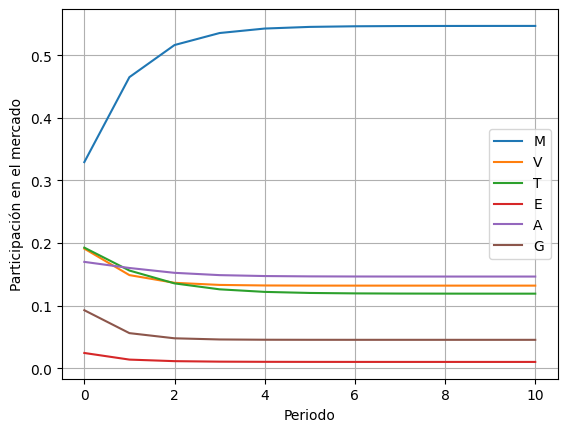
\includegraphics[width=1.0\textwidth]{../Images/RLExamples/MarketShare.png}
\end{frame}

\end{document}